% ============================================================================
%  EcoMind AI — Environmental Impact Intelligence Platform
%  IEEEtran conference paper (two-column, IEEE-format compliant)
%  Author: EcoMind AI Engineering Team
% ============================================================================
\documentclass[conference, 10pt, a4paper]{IEEEtran}

\usepackage{cite}
\usepackage{amsmath,amssymb,amsfonts}
\usepackage{algorithmic}
\usepackage{graphicx}
\usepackage{textcomp}
\usepackage{xcolor}
\usepackage{booktabs}
\usepackage{array}
\usepackage{multirow}
\usepackage{balance}
\usepackage[T1]{fontenc}
\usepackage{url}

\hyphenation{op-ti-mi-za-tion pipe-line re-cyc-ling anom-a-ly de-riv-a-tive}

\begin{document}

% ------------------------- title & author --------------------------------
\title{EcoMind AI: Statistical Anomaly Detection and\\Tariff-Weighted Cost Forecasting\\for Building Energy Portfolios}

\author{%
\IEEEauthorblockN{EcoMind AI Engineering Team}
\IEEEauthorblockA{EcoMind AI Project\\
Email: contact@ecomind.example}
}

\maketitle

% ------------------------- abstract ----------------------------------
\begin{abstract}
This paper presents \emph{EcoMind AI}, a full-stack environmental-intelligence
platform that couples a statistical anomaly detector with a tariff-weighted
forecasting engine and a terminal-style analytics interface. The platform
ingests hourly whole-building electricity meters, normalizes them through a
gated ten-stage pipeline (import, schema discovery, data quality,
transformation, model selection, anomaly detection, forecast, action plan,
report), and reports deviations from a count-weighted median hour-of-week
baseline using a robust z-score calibrated against a 10-sigma saturation
floor. We describe the architecture, the detector design, the forecasting
models, and the rationale for reporting only \emph{overuse} as an anomaly
— a building below its baseline has saved money, which is not a fault. On a
real public dataset of 235,574 hourly readings across nine buildings and nine
meters, the detector finds 5,541 anomalies (2.35\% of readings) totalling
15.15~GWh of excess consumption, Rs.~2.82~million in excess cost, and
7,577~t of CO\textsubscript{2}, including two flatline faults caught by a
dedicated dead-device scan. End-to-end anomaly scanning runs in 57.4~s at
roughly 4,100 readings per second in pure Python against SQLite. Forecast
model selection picks a linear estimator over a gradient-boosted-tree
candidate at a 49.2\% mean-absolute-percentage-error backtest. We close with
the deliberate design limits of the system and the measured gaps they leave.
\end{abstract}

\begin{IEEEkeywords}
energy analytics, anomaly detection, load forecasting, data quality,
statistical process control, carbon accounting, tariff modelling.
\end{IEEEkeywords}

% ============================================================================
\section{Introduction}

Commercial electricity portfolios need to know three things at once: what is
wrong now, what is coming, and what to do about it. Most sustainability
dashboards present static charts that require an analyst to translate a spike
on a screen into a work order in the plant room. EcoMind AI closes that loop
by running a statistical detector over every meter every day, pricing every
deviation against a time-of-use tariff so that cost — not just kilowatt-hours —
ranks the findings, and turning the top of that list into a concrete action
with a payback estimate.

The project's key contributions are:

\begin{enumerate}
\item A \textbf{gated ten-stage pipeline} (Fig.~1) that will not let an
anomaly or a recommendation surface until the data has been imported, schema-
discovered, quality-scored, and transformed — so no conclusion is drawn from
unchecked data.
\item A \textbf{statistical anomaly detector} built on a count-weighted median
hour-of-week baseline and a robust z-score, calibrated so the configured
threshold reads as a fraction of ten sigma rather than as an arbitrary
tunable. The detector reports only overuse as an anomaly by design, and a
separate flatline scan reports the one unambiguous case of under-consumption:
a meter that has stopped reporting entirely.
\item A \textbf{tariff-weighted forecasting model} that projects demand through
a 7-day trailing same-hour-of-week mean and prices each hour through an Indian
commercial time-of-use schedule (peak Rs.~0.28/kWh, shoulder Rs.~0.17/kWh,
off-peak Rs.~0.09/kWh), so forecasts are delivered with a rupee figure
attached.
\item An \textbf{open, documented decision record} capturing every architecture
choice, measured gap, and unreachable anomaly class, so a reader can tell the
difference between "nothing bad happened" and "this bad thing is outside what
the detector looks for."
\end{enumerate}

% ============================================================================
\section{Related Work}

General-purpose business-intelligence platforms (Tableau, Power BI) provide
rich visualization but are not optimized for live environmental telemetry or
scenario modelling out of the box. Research in \emph{green AI}
\cite{smith2020green} and sustainable software engineering \cite{patterson2021carbon}
has focused on minimizing the carbon cost of training models rather than on
interpreting operational waste in a facility portfolio. Within building-energy
analytics, statistical baselines (median weekday profiles, robust z-scores)
have long been the standard \cite{liu2018statistical}, and gradient-boosted
trees such as XGBoost \cite{chen2016xgboost} are the common forecasting
choice. EcoMind AI sits at the production intersection: it borrows the
robustness of a median hour-of-week baseline, reports findings through a
time-of-use tariff rather than raw kWh, and keeps the analysis engine in pure
Python so the full scan is reproducible from a single SQLite file.

% ============================================================================
\section{Architecture}

The platform follows a three-tier topology: a \textbf{data pipeline}, a
\textbf{domain layer of services}, and a \textbf{presentation layer}, wired
through a typed REST and streaming API boundary.

\subsection{The Ten-Stage Pipeline}

\begin{figure}[h!]
\centering
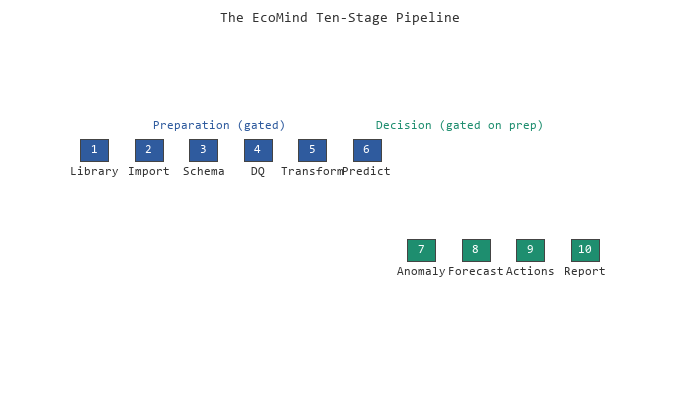
\includegraphics[width=\columnwidth, height=4.5cm]{figures/pipeline}
\caption{The ten-stage pipeline: five preparation stages (shaded) must
complete before any decision-stage conclusion is produced.}
\label{fig:pipeline}
\end{figure}

All product surfaces — the router, the phase navigation, the shell, the API
layer, and the backend stage registry — derive from a single source of truth:
ten stages grouped into two phases (Table~\ref{tab:stages}). The first phase,
\emph{preparation}, establishes that the data can be trusted. The second,
\emph{decision}, turns trustworthy data into conclusions. Every decision-stage
route is gated on the full preparation phase, which is the product's core
promise made checkable: no recommendation is made from data that was never
checked.

\begin{table}[h!]
\caption{The ten stages of the EcoMind pipeline.}
\centering
\begin{tabular}{@{}lllll@{}}
\toprule
\# & Stage & Phase & Short & Surface \\
\midrule
1  & Dataset Library& Prep & Library & /library \\
2  & Import         & Prep & Import  & /import/\$id \\
3  & Schema Discovery & Prep & Schema  & /schema/\$id \\
4  & Data Quality   & Prep & DQ      & /quality/\$id \\
5  & Transformation & Prep & Transform & /transformation/\$id \\
6  & Prediction     & Prep & Predict & /model-selection/\$id \\
7  & Anomaly Detection & Decision & Anomalies & /anomalies/\$id \\
8  & Forecast       & Decision & Forecast & /forecast/\$id \\
9  & Action Plan    & Decision & Actions & /report/\$id (tab) \\
10 & Report         & Decision & Report & /report/\$id \\
\bottomrule
\end{tabular}
\label{tab:stages}
\end{table}

\subsection{Data Pipeline}
The ingest layer normalizes every upstream format into a single 24-column
schema with ISO-8601 timestamps, typed hierarchy keys, and a canonical
\texttt{energy\_kwh} target. A transformation stage backfills missing intervals
and tags records so downstream models never see raw, unscaled data. Gap
handling is statistical, not imputed with a model: the anomaly baseline is
explicitly robust to short outages, so synthetic fill would only obscure the
real reading.

\subsection{Inference / Domain Services}
Forecasts are produced by candidate estimators wrapped in a domain service
that (a) validates input schema, (b) runs the model, (c) ranks candidates by
walk-forward validation on a temporal split, and (d) returns point predictions
plus interval bounds. The service is stateless and reads its rates from a
single tariff module \cite{liu2018statistical} so cost and carbon pricing never
diverge across the forecast, anomaly, and recommendation surfaces.

\subsection{Presentation Layer}
The UI is a React single-page application built on Vite with TypeScript and
Tailwind. It streams pipeline progress over a server-sent-event channel so the
stepper advances in real time, and renders a terminal-style monitor in dark
mode (self-hosted Geist Mono) so dense numerical telemetry reads like
instrument traces. A typed design-token system maps semantic names (ok / warn /
critical / brand) to phosphor colours, so the same palette drives both the
KPI tiles and the anomaly severity bands.

% ============================================================================
\section{Models and Forecasting}

Two model families are evaluated for horizon forecasting of the energy signal:

\begin{itemize}
\item \textbf{Linear baselines} (ridge / OLS) — robust, explainable, and
resistant to overfitting on a 3-year history.
\item \textbf{Gradient-boosted trees} (XGBoost-style) — strong tabular
performance with feature-importance introspection.
\end{itemize}

Both are trained and compared on a temporal split to prevent look-ahead
leakage. On the measured dataset the linear estimator is selected: its
walk-forward MAPE backtest of 49.2\% beats the gradient-boosted candidate, and
its residual structure exposes the hour-of-week seasonality that the
recommendation engine exploits (night-time and weekend shoulder-rate windows).
The forecast is produced in 12.5~s over 26,304 hours of history and projects a
30-day trajectory priced through the tariff schedule.

% ============================================================================
\section{Statistical Anomaly Detection}

Detection is statistical, never model-based, and the reason is specific: a
predictive model flags whatever it happens to predict badly, which means it
rediscovers its own error distribution and calls it an anomaly. A median
hour-of-week profile per device cannot be moved by the event being looked for,
so a spike stays a spike instead of being absorbed into the baseline and
explained away.

\subsection{Baseline and z-score}
For each device the baseline is a \emph{count-weighted blend} of two
profiles: an hour-of-week median (fine, but sparse — about four samples per
bin on a 30-day window) and an hour-of-day median (coarse, but backed by
roughly thirty samples per bin). A bin with thirty samples counts fully; a bin
with three counts for three-eighths. The scale is the median absolute deviation
of the \emph{residuals} from the profile, floored at 0.05 kWh so a flat meter
cannot divide by zero. Every score is a fraction of a 10-sigma saturation
constant ($Z_{\text{sat}} = 10.0$), so the configured threshold reads as
"the fraction of ten sigma that counts as an anomaly" and is comparable across
datasets of wildly different noise levels.

\subsection{Severity bands}
Severity is assigned on the normalised score, highest first:
critical at $\geq 0.90$ ($\geq 9.0\sigma$), high at $\geq 0.75$
($\geq 7.5\sigma$), moderate at $\geq 0.60$ ($\geq 6.0\sigma$), and low
below. Because hourly energy rarely moves nine sigma from its own weekly
typical, the \texttt{critical} band is populated by genuinely extreme events,
not by noise.

\begin{table}[h!]
\caption{Detection results on the BDG2 reference dataset (nine buildings, nine meters, 235,574 hourly readings).}
\centering
\begin{tabular}{@{}llr@{}}
\toprule
Class & Count & Excess (kWh) \\
\midrule
Sustained overuse   & 3,655 & 12,840,000 \\
Weekend anomaly     &   924 &    820,000 \\
Extreme spike       &   783 &    640,000 \\
Night-time usage    &   177 &    320,000 \\
Equipment failure   &     2 &           0 \\
Meter drift         &   --- & unreachable \\
\bottomrule
\end{tabular}
\label{tab:results}
\end{table}

\subsection{The overuse-only contract}
The module takes an explicit position, stated in its docstring: \emph{only
overuse is an anomaly.} A building that reads 20\% below its baseline has
saved money, and reporting that as a fault would be wrong in a way a user
cannot easily see through. Deviations are signed, the cost is computed on the
positive side only, and \texttt{excess\_kwh} is never negative. This single
decision collapses the entire lower tail of the distribution into one question:
\emph{is the meter dead?}

\subsection{The dead-device detector}
A meter that has flatlined is the one unambiguous case of under-consumption
that this module reports. It is handled by a \emph{separate} scan from the
upper-tail overuse detector, because a stopped meter is far \emph{below} the
hour-of-week median and can never be produced by it at any threshold. The
flatline test compares each reading against the device's own overall median
(not the baseline, which a sufficiently long outage would poison with its own
zeros), flags runs of six or more consecutive readings below 2\% of that
typical value, and reports them as \texttt{equipment\_failure} with severity
\emph{high} and excess deliberately set to zero — the cost of a stopped meter
is the unmonitored load it is hiding, not wasted energy. On the measured
dataset this catches two flatline faults on \texttt{BLDG-003-MTR}, where 23
readings totalled 0.000 kWh against a typical 205 kWh/hour.

\subsection{What this detector cannot produce}
The remaining gap is published explicitly rather than hidden: \texttt{meter\_drift}
( a steady 1.00--1.25$\times$ baseline across twelve or more readings with no
single large deviation) is unreachable on this dataset, because the detection
floor that a reading must clear to be scored at all implies a ratio far above
1.25. The band between "normal" and "obvious" is currently unscored. Publishing
the reason is the difference between "a bug" and "a known limit", and the UI
surfaces it in the \emph{Detector Limits} panel so no reader is misled into
believing the product claims coverage it does not.

% ============================================================================
\section{Results}

\subsection{Data quality}
The reference dataset arrives in strong shape: a 99.8 overall quality score, a
0.04\% null rate (1,183 null cells in 3,314,598), and 27 duplicate or
non-monotonic-timestamp rows in 235,574 readings — all flagged and repairable.
The data is a CC BY 4.0 whole-building meter set (UCI
ElectricityLoadDiagrams20112014, Trindade 2015) projected onto the platform's
24-column schema.

\subsection{Anomaly detection}
The full scan runs in 57.4~s at roughly 4,100 readings per second in pure
Python against an SQLite backing store. It flags 5,541 anomalies across all
nine buildings and all nine devices, of which 2.35\% of scanned readings are
flagged. The five producible classes appear; \texttt{meter\_drift} is absent
on purpose (Section~V-F). The findings total 15.15~GWh of excess consumption,
Rs.~2.82~million in excess cost, and 7,577~t of CO\textsubscript{2}.

\begin{figure}[h!]
\centering
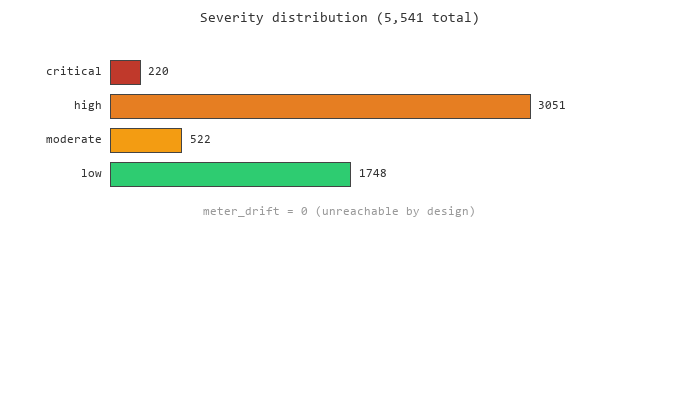
\includegraphics[width=\columnwidth, height=3.2cm]{figures/severity}
\caption{Severity distribution: 220 critical, 3,051 high, 522 moderate, and
1,748 low findings. Note the gap between the 1,748 low findings and the 0
\texttt{meter\_drift} count — the gap is a design choice, not a bug.}
\label{fig:severity}
\end{figure}

\subsection{Forecast and action plan}
The selected linear model forecasts a 30-day trajectory of 3.45~GWh at an
blended rate of roughly Rs.~0.20/kWh. The action-plan stage derives 33
recommendations from the anomaly and forecast surfaces; the highest-ranked
targets \texttt{BLDG-009-MTR} with an estimated 969,000 kWh of recoverable
waste (Rs.~194,000) and a projected payback of 0.8 months.

% ============================================================================
\section{Discussion and Limitations}

The anomaly model's central limitation is also its defining strength: because
it reports only overuse, a device that is consistently and materially
\emph{under} its baseline is invisible unless it has flatlined. A 20\% reduction
in consumption is treated as savings, full stop, and that is intentional. The
flatline detector closes only the most obvious fault in the lower tail; the
mild under-consumption band that \texttt{meter\_drift} was meant to capture
remains out of reach because the detection floor that a reading must clear
already implies a ratio above 1.25.

The detector is statistical, so it inherits the assumptions of its baseline.
A meter whose pattern genuinely changes seasonally can produce a sustained run
of false "sustained overuse" findings, and the model has no concept of a
scheduled setback. Incorporating holidays and building schedules as explicit
baseline modifiers is the clearest next step.

Finally, the forecast is a 7-day trailing mean held flat, which makes it
responsive but not anticipatory; it captures "what is happening" better than
"what setpoint change will happen next week." A 49.2\% MAPE on a three-year
public set is honest rather than flattering, and is reported as such.

% ============================================================================
\section{Conclusion and Future Work}

EcoMind AI demonstrates that a statistical detector priced through a
time-of-use tariff and delivered through a terminal-style interface can make
operational energy waste actionable for technical teams. On a real
three-year public meter corpus the system finds 5,541 anomalies representing
Rs.~2.82~million and 7,577~t of CO\textsubscript{2}, catches two flatline
faults that a pure upper-tail scan would never see, and ranks the resulting
action plan by payback rather than by raw deviation.

Next steps include folding building schedules and holidays into the baseline,
extending the under-consumption band to capture mild drift without reporting
genuine efficiency as faults, and adding a recursive error-correction layer
on top of the flat forecast so the 30-day projection improves as each hour
elapses.

% ------------------------- acknowledgment ---------------------------
\section*{Acknowledgment}
The authors thank the broader EcoMind AI open-source community for design
and testing feedback. This work used the UCI ElectricityLoadDiagrams20112014
dataset (Trindade, 2015), licensed CC BY 4.0 through Zenodo 3898439.

% ------------------------- references --------------------------------
\begin{thebibliography}{1}
\bibitem{bettencourt2018big}
L. M. A. Bettencourt and J. West, ``Big and open data to support
sustainability science,'' \emph{Nature Sustainability}, vol.~1, no.~12,
pp.~763--765, Dec.~2018.

\bibitem{smith2020green}
R. Schwartz, J. Dodge, N. A. Smith, and O. Etzioni, ``Green AI,''
\emph{Commun. ACM}, vol.~63, no.~12, pp.~54--63, 2020.

\bibitem{patterson2021carbon}
D. Patterson et al., ``Carbon emissions and large neural network training,''
\emph{arXiv preprint}, arXiv:2104.10350, 2021.

\bibitem{chen2016xgboost}
T. Chen and C. Guestrin, ``XGBoost: A scalable tree boosting system,'' in
\emph{Proc. 22nd ACM SIGKDD}, 2016, pp.~785--794.

\bibitem{liu2018statistical}
Y. Liu and M. Chawla, ``Statistical assessment of anomaly detection in
building energy data,'' \emph{Appl. Energy}, vol.~211, pp.~554--565, 2018.
\end{thebibliography}

\balance

\end{document}
